\chapter{System Architecture and Implementation}
\label{chap:archi}

Our main contribution in this paper is the creation of a brand action recognition algorithm. In this chapter, we will give a precise step-by-step description of our system.
\section{Hardware and Framework}
In this section, we will describe the hardware from which we obtained our data and the software elements that support our work.
\subsection{ROS Architecture}
Our algorithm is supposed to be applied on any domestic robot, and can become part of a larger robot control software. To make it portable and easy to plug to larger projects, we implemented it to be fully compatible with ROS.

ROS \cite{ROS} - for Robot Operating System - is not really a proper OS but rather a middleware that run on most Linux distributions whose primary task is to provide a robust support for large volumes of data that need to be processed in real time. It also makes it possible to paralellize a lot of programs even if some of the hardware does not have high performance CPU or GPU.

The basic principle of ROS is that it makes all the different programs work as nodes in a network. The most powerful computer of the network - in our case a desktop PC - hosts the ROS Core node and acts as a server: it is responsible for managing the exchange of data among all the other nodes. Each ROS node can do three basic actions: it can publish its output at a specified rate as ROS topics, which are then advertised by the Core node. It can also subscribe to topics published by other nodes, and can therefore use this data as real-time input for its own computations. Finally, it can propose ROS services to other nodes, which means that other nodes can exceptionally ask it for a specific data that is not published. 

The code for each node can be written in either C++ 11 or Python 2.7, and ROS can therefore also be useful to link the advantages of these two languages in one software. On this project, the computationally expensive code is written in C++ for its rapidity and the code for managing the data and transforming it is written in Python to make use of Numpy and other useful modules.

The ROS architecture is really robust for robotics since the computer that hosts the Core node can take care of the heavy computation tasks while the limited robot computer only has to send data to the network and get back the responses. Another big advantage of ROS is that it is extremely modulative: the hardware may change completely or you may add another or even ten robots to the system and all you have to do is to make sure that every node publishes and subscribes to the good topics. For all of these reasons, we chose ROS so that our software can be effective in many different environments with only little adaptation.

\subsection{Turtlebot}
The robot we used for our research is a Turtlebot2\footnote{https://www.turtlebot.com/turtlebot2/}. Turtlebot\textsuperscript{TM} is an easily programmable robot which consists in a Kobuki\footnote{http://kobuki.yujinrobot.com/about2/} base on top of which is mounted a Microsoft Kinect\textsuperscript{TM} sensor. 

The Kobuki\textsuperscript{TM} base contains four wheels including two motorised ones. A Kobuki\textsuperscript{TM} robot can rotate around itself and move forward and backward. The wheels provide odometry information - which will be useful for the mapping process - and the base also contains collision sensors.

The Kinect\textsuperscript{TM} sensor is the combination of a RGB camera and a IR sensor. The first version of the Kinect sensor also provides a Windows\textsuperscript{TM} development environment, but this is incompatible for ROS, which only runs on Linux. Because of that, we decided to use the second version instead: Kinect for XBox One\textsuperscript{TM}, since this version provides more accurate results\cite{kinect_comparison}. However, since there is no official driver release for this sensor, we instead use an open source one named Freenect2\cite{libfreenect2}, which provides us both RGB and IR images, but no depth registration. Further explanation about the depth registration process and point cloud publication will be given later on this chapter.

We then use a program called kinect2 bridge\cite{iai_kinect2} to reconstruct the point cloud from the RGB and IR images. This is done by performing depth to color frame registration using extrinsic parameters of the Kinect cameras\footnote{\raggedright A description of the algorithm used can be found here: http://nicolas.burrus.name/index.php/Research/KinectCalibration}.
It then publishes 

\section{Unsupervised Pose Clustering}
In this section we describe how we obtain the pose estimation and create a cluster model from them.

\subsection{Choice of input dimension}
When we designed our workflow, we had to make a choice between estimating human action either from 2D or 3D human pose estimation. The tradeoff between the two techniques can be found in table \ref{tab:dimension_comparison}.

3D is a more natural environment for the robot since it already uses this coordinate system for mapping and navigation purpose. It also makes object segmentation easier since 3D point cloud data is sparse as opposed to images, we will detail that point in section \ref{section:object_seg}.

On the other hand, using 2D input is less computationally costly, and there are quick and reliable algorithm to perform body pose estimation like OpenPose, that we will describe in section \ref{section:openpose}. Another big advantage of 2D input is that image or video datasets are a lot easier to find than point cloud datasets. Because of all of these points, we decided to perform the clustering on 2D pose inputs.

\begin{table}[h]
    \centering
    \caption{Comparison of features between 2D and 3D environment}
    \label{tab:dimension_comparison}
    \begin{tabular}{|l|l|}
        \hline
        2D environment & 3D environment \\ \hline
        \textbf{+ Many image/video datasets available} & -- Datasets are rare \\
        + Easy to compute input & -- Computationally costly \\
        + Same algorithm for both human & -- Separate algorithms for the two tasks \\ detection and pose estimation & \\
        -- One dimension is not used & + Robot environment is in 3D \\
        -- Unsupervised object clustering: tricky & \textbf{+ Unsupervised object clustering} \\
        & \textbf{~~is easier (sparsity)}
        \\ \hline
    \end{tabular}
\end{table}

\subsection{2D Human Pose Estimation}
\label{section:openpose}
Human pose estimation is performed by using a trained deep learning model named OpenPose \cite{Openpose}. It takes image input and processes the body joint position for each individual present on the scene by computing part affinity field (PAF) fields. OpenPose performs quick enough for real-time applications: about 10 frames per second on our desktop PC. The outputs for each frame consists in the list of humans detected, where each human is represented as the list of his 18 body joints position as shown in fig \ref{fig:2D_joints_vis}. Each point consist in x and y coordinates of the joint on the image and a score confidence which represent the confidence the algorithm puts into this result. This confidence score will prove itself useful in the next steps of our algorithm.

In order to generate body poses to use them as input data for the pre-training model described in section \ref{section:SOINN}, we use the publicly released OpenPose demo with previously selected images from our pre-training dataset. For the real-time learning this solution is longer viable because of its computational cost, and we developed our own ROS node based on the OpenPose API that subscribes to the RGB image published by the kinect2 bridge node and publishes the OpenPose output in return. This solution runs at around 10 FPS.

\begin{figure}[ht]
    \centering
    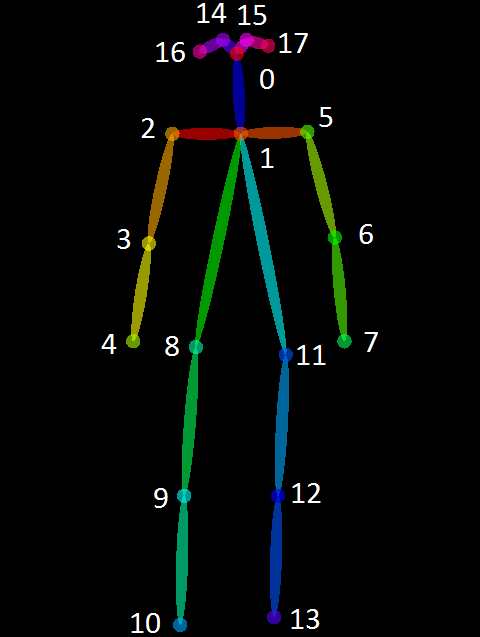
\includegraphics[width=80mm, keepaspectratio]{images/2D_body_joints_visualisation.png}
    \caption{2D human body joints visualisation}
    \label{fig:2D_joints_vis}
\end{figure}

\subsection{Unsupervised Clustering}
\label{section:SOINN}
Most of unsupervised learning algorithms can be applied to pose estimation. In theory we could use as input anything, and we particularly considered using methods such as the classical and very simple K-means \cite{k_means} to more complete models such as self-organizing map \cite{self_organizing_map} or neural gas clustering \cite{neural_gas}.

However, we considered that an online algorithm would be better for our application, since it is more in accordance to a domestic robot environment: the robot should never stop learning to adapt itself constantly to the changes to the changes in its environment. Even with that constraint, a lot of different methods exist \cite{online_clustering_algo}, but in the end we decided to use the Self Organizing Incremental Network (SOINN) \cite{SOINN} to deal with our task. We chose this algorithm mostly because it is lightweight, operates in real-time and tackles efficiently the Stability-Plasticity Dilemma \cite{stability-plasticity_dilemma}. 

\begin{figure}[h]
    \centering
    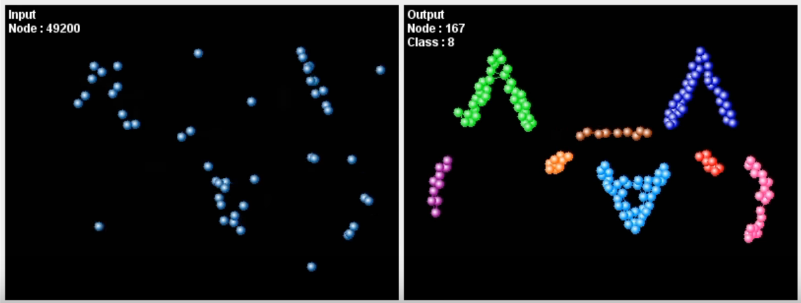
\includegraphics[width=150mm, keepaspectratio]{images/SOINN_cat.png}
    \caption{SOINN algorithm applied to noisy artificial data. For each step, random points from the original figure are selected along with pure noise points(left image). The algorithm assigns each new signal to a cluster, called node and reconfigure its architecture by recomputing its nodes values and the relationship between them (right image).}
    \label{fig:SOINN_cat}
\end{figure}

SOINN takes as input vectors of any dimensions - the only restriction is that these dimensions should remain consistent over time - and based on the distance between this new signal and the existing nodes either assigns the signal to an existing node or creates a new one. It then reconfigure its architecture and may decide to destroy nodes not used anymore or to fuse two nodes near to each others.
An example of clustering on artificial data is shown in figure \ref{fig:SOINN_cat}. A complete description of the algorithm can be found in pages 49 to 55 in \cite{SOINN}. In this research, we used the implementation from \cite{soinn_implementation} for pose clustering, and we modified it to make it an ROS node able to modify the volume of its input in order to perform pose/interaction clustering as described in section \ref{section:pose-interaction_clustering}.

For our particular application, we use SOINN twice in our workflow. The first time is during the pre-training step, where we make SOINN learn to cluster 2D body poses that OpenPose generated from a dataset described in chapter \ref{chap:experiments}, which generate what we call a naive pose estimation. This first estimation will be useful as a foundation for our proposed model: indeed since images/video datasets are easy to find and OpenPose can quickly generate body pose estimations based on them, the training data is abundant. Later on, when the robot is operated in real-time, we will transfer the knowledge it gained on 2D body pose estimation to create another modified SOINN model from this original model using to include the human/object interaction along with the pose estimation. This particular step will be described in details in section \ref{section:pose-interaction_clustering}.

\subsection{Pre-training - to be completed}
In this section, we will explain the pre-processing ...

For our application, we decided to discard the joints number 14 to 17 corresponding to the right/left eye and ears respectively. These joints did not affect the clustering result and were often either not detected at all or with a bad confidence score, which is problematic for the preprocessing part of our pose clustering algorithm.

\section{Spatial Context Acquisition}
In this section, we will describe the different tools we used to make the robot able to perform environment mapping and object segmentation on this map.

\subsection{Simultaneous Localization and Mapping, Navigation}
Making the robot aware of its environment is a difficult but well-studied problem. It can be divided into two distinct tasks, where the robot needs to answer two questions:
\begin{itemize}
    \item{What does my environment look like ? $\Rightarrow$ Mapping}
    \item{Where am I ? $\Rightarrow$ Localization}
\end{itemize}

These two tasks used to be performed separately, but current state of the art algorithms now tackle them both at once: this is called Simultaneous Localization and Mapping (SLAM). For our project, we will use the rtabmap SLAM algorithm described in \cite{rtabmap}, winner of the IROS 2014 Kinect Challenge. Its greatest feature is that it can detect loop closure to successfully update its map in real time to avoid point cloud overlap.

In the original work, the algorithm only used Kinect data to reconstruct visual odometry from it, but since the turtlebot is already able to compute its odometry from its wheels rotation sensors, we used that mechanical odometry instead to increase performance and reduce computation cost. We used for our project a modern ROS implementation of rtabmap, which also generates 2D floor-projected collision map from the 3D point cloud map, and compute path planning from this map and the robot localization, based on \cite{rgbd-slam}\cite{loop-closure}.

\subsection{3D Object Segmentation}
\label{section:object_seg}
In this section, we will explain how we perform 3D object segmentation using the environment map generated in the previous section as input. We developed entirely the programs in this section by using the C++ Point Cloud Library (PCL) \cite{PCL}.

Object segmentation is one of the major problems in computer vision, and performing it in 2D in an unsupervised way is still unattainable. Hopefully, this problem is far more easier in 3D, where data is sparse and simple algorithms can attain quite good results. Moreover, the problem of detecting human/object interaction is also really difficult in 3D while being trivial in 2D. This is the main motivation for performing this part of the workflow in 3D even if our clustering algorithm was previously trained on 2D examples.

The first problem that arise when trying to deal with our map is that it is far too heavy to carry real-time operations - the raw map is about 40M 3D colored points. We therefore begin by reducing that number by applying the following operations: 

\begin{description}
    \item[Cropping of farthest points] Points that are too far away from the median depth are suppressed from the cloud. These noisy points are artifacts generated by a local error in depth estimation and are pointless for our study.

    \item[Downsampling] We reduce the number of points in the point cloud by creating a voxel grid, and fusing the points in each voxel into a new point whose coordinates are those of the voxel centroid. This technique is interesting since it reduces the amount of data for near objects where the point cloud is dense and information is redundant, and leaves almost untouched distant objects that are already less dense and were each point brings a lot of information.

    \item[Walls detection and extraction] For each axis, we detect the walls as the largest plane normal to that axis with 20$^\circ$ tolerance and remove them. Plane detection is done using the RANSAC algorithm \cite{RANSAC}, and no extraction is performed if that detected plane is too small, for it can mean that no wall is present on the image and another object was detected instead.

    \item[Transformation of the data into a Kd-tree] PCL point cloud are an unordered data structure by default, and can simply be accessed by calling their index ranging from 0 to the point cloud size. While this characteristic makes them very convenient to manipulate to apply simple algorithms on them, it considerably slows down the process when an algorithm iterates several times on it. To speed up the next steps, we convert our raw point cloud data into a Kd tree representation structure.
\end{description}

After these steps, the remaining point cloud size is in the order of 10 000 points, which is much more reasonable for real-time processing. We can then carry out object segmentation on it by using the Euclidean cluster extraction algorithm \cite{euclidean_cluster_extraction}. This type of segmentation performs well in extracting objects that are well-separated in the point cloud. However, it is not able to differentiate between objects that are touching each others, like several books on the same pile for example. Other types of segmentations can be used to tackle this problem, such as the Region growing segmentation algorithm \cite{region_growing_seg}. This technique is able to differentiate adjacent objects based on their mean curvature, however based on our test it tends to be too strict on its detection, which ends in one object being detected as several ones. 

An ideal approach would be to average the result of several segmentation algorithm to obtain a fine-tuned object segmentation, but this method is very computationally expensive and does not scale well for real-time applications. Therefore, we prefer to use euclidean cluster extraction since it runs more quickly and identifies a reasonable number of objects. Of course, using more complex object segmentation algorithms that can run in real-time in the future may improve the results of our technique, and me valuable as a future work.

\subsection{3D Pose Estimation}
In order to detect the human/object interaction, we do not only need the object position information, but also the position of the human pose estimate in the same coordinate system. OpenPose only provides the pixel locations of body joints position on a 2D image, so we need to transform that output by estimating the real-world coordinates of each point.

To that end, we developed a ROS node that subscribes to both the 2D ($x_{pixel}, y_{pixel}$) body skeleton published by the ROS OpenPose node in the image coordinate and the 3D point cloud. It then computes the real world coordinates ($x_{world}, y_{world}, z_{world}$) coordinates of each body part based on the average real-world coordinates of its neighbouring points on the image. A precise description of the algorithm can be found as algorithm \ref{alg:openpose3d}.

\begin{algorithm}[h]
    \KwData{(synchronized)\\2D image coordinates of a body joint: ($x_{pixel}, y_{pixel}$) \\ point cloud environment: cloud}
    \KwResult{3D real-world coordinates of that body joint: ($x_{world}, y_{world}, z_{world}$)}
    get synchronized input \\
    get image width w, image height h \\
    possible\_x, possible\_y, possible\_z $\leftarrow$ \O, \O, \O \\
    \If{$x_{pixel}$ is NaN or $y_{pixel}$ is NaN}{($x_{world}, y_{world}, z_{world}$) $\leftarrow$ (NaN, NaN, NaN)}
    neighbours\_indexes $I_n$ $\leftarrow$ \O \\
    \ForEach{neighbour($x_{i}, y_{i}$) in a 3$\times$3 window around body joint}{ADD $width \cdot y_i + x_i$ TO $I_n$}
    \ForEach{indice i in $I_n$}
    {\If{cloud[i] is valid}
    {ADD cloud[i][x] TO possible\_x \\
    ADD cloud[i][y] TO possible\_y \\
    ADD cloud[i][z] TO possible\_z}
    $x_{world} \leftarrow average(possible_x)$ \\
    $y_{world} \leftarrow average(possible_y)$ \\
    $z_{world} \leftarrow average(possible_z)$}
    \caption{3D Human Pose reconstruction for one body joint}
    \label{alg:openpose3d}
\end{algorithm}

\section{3D Human-Object Interactions}
In this part, we will describe how we detect human/object interaction and how we adapt our pre-trained SOINN model to make it use these interaction as additional input.

\subsection{Interaction Detection}
In this work, our detection method is pretty straightforward. We simply define an interaction when one or more of the human body joint either touches or enters into the bounding box of a detected object. In order to conserve OpenPose multi-human detection ability, we define the data structure of an interaction as the combination of a OpenPose ROS human list and an object list. In that way, we are able to track human/object interaction in real-time no matter how many humans interact with any number of objects.

\subsection{Pose-Interaction Clustering}
\label{section:pose-interaction_clustering}
There are many ways to include the human/object interaction as an additional information to differentiate clusters issued by SOINN. We finally decided to integrate it as a new dimension for both existing and future SOINN nodes. By doing that, we take advantage of the SOINN algorithm to adapt itself to new data without having to change drastically core functions which would have lead to a completely new algorithm in the end, instead of refining the existing one.

The main idea is to create a new SOINN model from our existing one. The nodes of this model have one more dimension than previously: added to the 28 first coordinates that represent the 2D pose coordinates for one person, we add the object id associated with this pose. Since this id ranges from 0 to the number of detected object -- 1, we initialize the last coordinate of our previous nodes to --1. 

A new signal is given to the algorithm as input each time that a new interaction is detected, and therefore contains both the body pose and human/object interaction informations. From there, another problem that arise is that it is no longer possible to compute the distance between new signals and existing nodes as we did before. Indeed, classical SOINN algorithm uses euclidean distance but our last coordinate is of course incompatible with that distance. 

We propose to compute the distance between our new vectors as the previous euclidean distance between them from which we add a penalty if the two objects are associated with different objects or subtract a constant as a bonus if they are associated with the same object. If one of the two compared signal is not associated with an object yet, ie its last coordinate is --1, we just compute the euclidean distance like before.